\chapter{Trabalhos Relacionados}
\label{cap:trabalhos-relacionados}

Este capítulo revisa os modelos de processos pontuais baseados em Transformer que antecedem e fundamentam o HoTHP, além das técnicas de extrapolação de comprimento que motivam sua proposta. Aqui partimos do Transformer Hawkes Process (THP) e do RoTHP, que substitui o \textit{encoding} temporal absoluto por \textit{rotary position embeddings}. Por fim, discutimos o problema de \textit{length extrapolation} e a noção de viés indutivo de recência, que conecta esses modelos ao kernel de Hawkes e dá origem à abordagem proposta nesta dissertação.

\section{Transformer Hawkes Process (THP)}\label{sec:thp}

    A arquitetura de Transformers \cite{vaswani_attention_2017} mostrou que utilizar Atenção pode oferecer bons avanços em relação ao uso de redes neurais recorrentes, porém, como RNNs tradicionais, os Transformers também foram projetados para eventos discretos, como as palavras de uma frase. \citeonline{zuo_transformer_2021} tiveram que modificar a arquitetura transformando-a em continua, assim como \citeonline{mei_neural_2017} tiveram que fazer, ao transformar a LSTM tradicional em Continuous Time-LSTM.

    Em problemas de tradução, que foram originalmente a primeira aplicação dos Transformers, a ordem das palavras basta, sem necessidade de precisão além dessa. Porém, em análises de processos pontuais precisamos saber o momento em que cada evento ocorre. Para resolver esse problema, \citeonline{zuo_transformer_2021} propuseram um encoding temporal, representado pela Equação~\ref{eq:temporal-encoding-thp}, onde o argumento não é a posição (discreta), como proposto por \citeonline{vaswani_attention_2017}, e sim o timestamp $t_j$:
    \begin{equation}
        [z(t_j)]_i = 
        \begin{cases}
            \cos \left( \frac{t_j}{10000^{\frac{i-1}{M}}} \right), & \text{se } i \text{ é ímpar,} \\
            \sin \left( \frac{t_j}{10000^{\frac{i}{M}}} \right), & \text{se } i \text{ é par.}
        \end{cases}
        \label{eq:temporal-encoding-thp}
    \end{equation}
    
    A Equação \ref{eq:temporal-encoding-thp} utiliza funções trigonométricas para determinar um encoding temporal para cada timestamp, ou seja, para cada $t_j$ é computado de forma determinística $\mathbf{z}(t_j) \in \mathrm{R}^M$, onde $M$ é o tamanho da dimensão do encoding. Além do enconding temporal, é utilizado também uma camada de embedding, matriz $\mathbf{U}$, para os diferentes tipos de eventos. Os embeddings são então representados por $\mathbf{X=(UY+Z)}^T$, onde $\mathbf{Y}$ é a coleção one-hot encoding de tipos de eventos e $\mathbf{Z}$ a matriz com os vetores $\mathbf{z}$ concatenados. Após as camadas de embeddings, $\mathbf{X}$ é passado por um mecanismo de auto atenção como mostrado a seguir:
    \begin{equation}
        \mathbf{S} = \text{Softmax} \left( \frac{\mathbf{Q} \mathbf{K}^{\top}}{\sqrt{d_k}} \right) \mathbf{V}, \quad \text{onde } \mathbf{Q} = \mathbf{X} \mathbf{W}^Q, \mathbf{K} = \mathbf{X} \mathbf{W}^K, \mathbf{V} = \mathbf{X} \mathbf{W}^V.
        \label{eq:scaled-dot-product-attention-full}
    \end{equation}

    $\mathbf{Q}$, $\mathbf{K}$ e $\mathbf{V}$ são as matrizes Query, Key e Value obtidas através de transformações em $\mathbf{X}$ e $\mathbf{W}^Q$, $\mathbf{W}^K$ e $\mathbf{W}^V$ são pesos de transformações lineares. Então, $\mathbf{S}$ passa por uma rede feed forward gerando $\mathbf{h}(t)$:
    \begin{equation}
        \mathbf{H} = \text{ReLU}(\mathbf{SW}_1^{FC} + \mathbf{b}_1)\mathbf{W}_2^{FC}+\mathbf{b}_2, \quad \mathbf{h}(t_j)=\mathbf{H}(j,:).
        \label{eq:scaled-dot-product-attention-full}
    \end{equation}

    \begin{figure}[h!]
        \centering
        \captionsetup{width=10cm}%Da mesma largura que a figura
        \Caption{\label{fig:thp}Arquitetura do Transformer Hawkes Process} \UFCfig{}{
        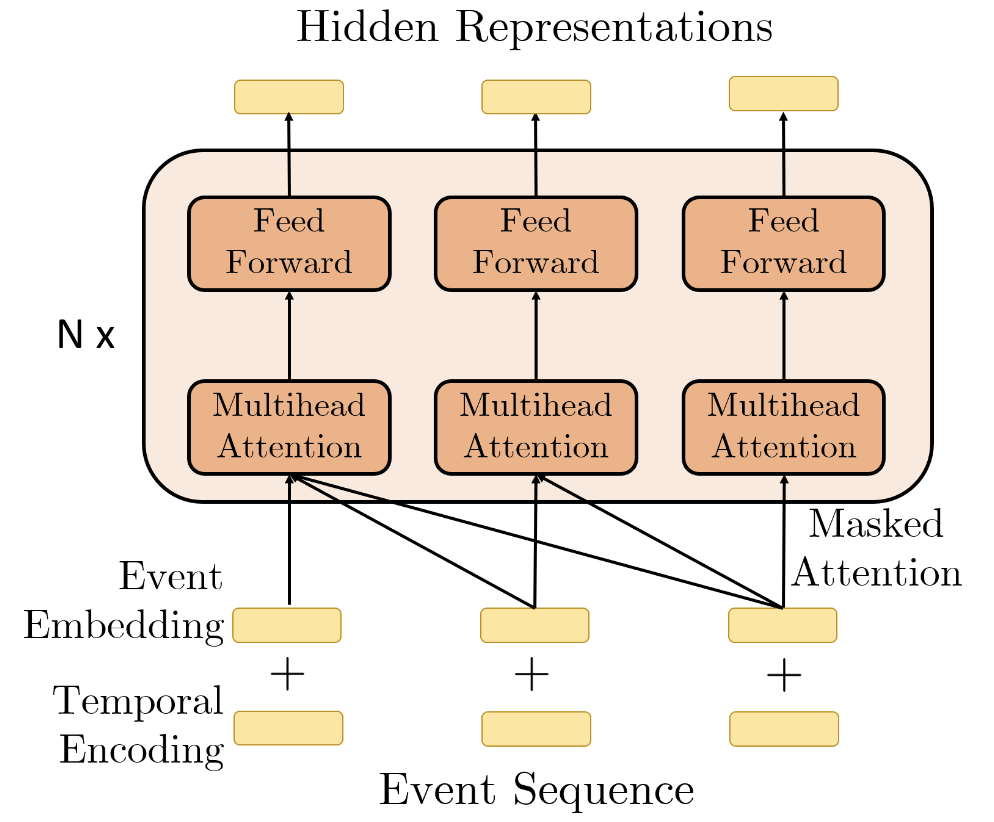
\includegraphics[width=10cm]{figuras/figura-thp.png}
        }{
            }	
    \end{figure}

    \citeonline{zhang_self-attentive_2020} \gls{SAHP} propuseram um calculo diferente para o temporal encoding. Ao contrário do THP que utiliza apenas o timestamp $t_i$, o SAHP desloca (shift) o evento para uma nova posição $i'$, utilizando tanto a posição $i$ quanto o timestamp $t_i$, que é calculada com $\mathrm{sin}(\omega_k \times i + w_k \times t_i)$, onde $\omega$ é a frequência angular e $w$ é um parâmetro de escala, ajustado pelo modelo, que converte o timestemp $t_i$ para um deslocamento de fase, dentro da função senoidal (como em outros modelos, o Self-Attentive Hawkes Process usa seno para eventos pares e coseno para eventos ímpares).
     
    A Figura \ref{fig:thp} mostra a arquitura do Transformer Hawkes Process. Cada sequência de eventos passa por duas camadas de embeddings e multiplas vezes por módulos de multi-head self attention. 

    \begin{equation}
        \lambda(t \mid \mathcal{H}_t) = \sum_{k=1}^K \lambda_k (t \mid \mathcal{H}_t)
        \label{eq:thp-lambda}
    \end{equation}
    
    Como vimos anteriormente, após todo o processo de embedding, atenção e rede feed-forward, é gerado, finalmente, $\mathbf{H}$, que faz com que possamos calcular o $\lambda_k$, necessário na Equação \ref{eq:thp-lambda}. O cálculo da intensidade para cada tipo de evento é dado por: 
    \begin{equation}
        \lambda_k(t \mid \mathcal{H}_t) = f_k \left(
        \underbrace{\alpha_k \frac{t - t_j}{t_j}}_{\text{corrente}}
        + \underbrace{\mathbf{w}_k^\top \mathbf{h}(t_j)}_{\text{histórico}}
        + \underbrace{b_k}_{\text{inércia}}
        \right)
        \label{eq:htp-thp-lambdak}
    \end{equation}

    Na Equação \ref{eq:htp-thp-lambdak}, a primeira parte "corrente" é uma interpolação entre $t_j$ e $t_{j+1}$ onde $\alpha$, que é um elemento aprendido, modula a importância dessa interpolação. A segunda parte utiliza o histórico $\mathbf{h}(t)$ dos eventos e o último elemento $\beta_k$ representa o estado estacionário, onde a probabilidade do próximo evento não é influenciada pelo histórico de eventos.
    
        
\section{Rotary Position Embeddings (RoPE) e o RoTHP}\label{sec:rothp}

    Vimos que o uso de RNNs possuem limitações tanto para memória de eventos distantes como no próprio treinamento da rede, pois cada evento precisa ser processando antes do próximo evento, já que leva o estado do evento anterior. Através do mecanismo de atenção, modelagens usando Transformers resolvem esses dois problemas, porém, a maioria das implementações não são resilientes à ruídos nos dados (timestamps). Em datasets reais, a presença de tais ruídos é muito comum, principalmente em função de atrasos físicos na gravação do timestamp. Por exemplo, em redes wireless, os rispositivos registram eventos mesmo sem estarem com seus relógios perfeitamente sincronizados entre si, fazendo com que haja discrepância no dataset final. O THP e suas variantes mais comuns adotam encoding temporal senoidal, ignorando tais características dos dados.  
    
    \citeonline{su_roformer_2023} demonstraram que o calculo da verossimilhança utiliza apenas a diferença dos tempos dos eventos e, dessa forma, propuseram utilizar as distâncias relativas entre os tokens em modelos de linguagem, substituindo o temporal encoding, da arquitetura tradicional de Transformers, pelo tempo relativo, dentro do mecanismo de atenção. Para isso, utilizamos o vetor de input (embedding) por pares ($d_i$, $d_{j+1}$). Cada par passa por uma matriz de rotação 2D gerando uma matriz de rotação $\mathbf{R}$, onde $\Theta = \{ \theta_j = 10000^{-2(i-1)/d}, i \in [1,2,..., d/2]\}$ fazendo $f_{\{q,k\}}(\mathbf{x}_m, m)=\mathbf{R}_{\theta, m}^d\mathbf{W}_{\{q,k\}}\mathbf{x}_m$, onde $q$ e $k$ são os componetes Query e Key do mecanismo de atenção:
    \[
        R_{\Theta,m}^d =
        \begin{pmatrix}
        \cos(t_i \theta_1) & \sin(t_i \theta_1) & 0 & 0 & \cdots & 0 & 0 \\
        -\sin(t_i \theta_1) & \cos(t_i \theta_1) & 0 & 0 & \cdots & 0 & 0 \\
        0 & 0 & \cos(t_i \theta_2) & \sin(t_i \theta_2) & \cdots & 0 & 0 \\
        0 & 0 & -\sin(t_i \theta_2) & \cos(t_i \theta_2) & \cdots & 0 & 0 \\
        \vdots & \vdots & \vdots & \vdots & \ddots & \vdots & \vdots \\
        0 & 0 & 0 & 0 & \cdots & \cos(t_i \theta_{d/2}) & \sin(t_i \theta_{d/2}) \\
        0 & 0 & 0 & 0 & \cdots & -\sin(t_i \theta_{d/2}) & \cos(t_i \theta_{d/2})
        \end{pmatrix}.
    \]

    A Figura \ref{fig:rope} ilustra os tokens de um modelo de linguagem, o vetor de posicionamento e como o RoPE utiliza pares do embedding para aplicação rotação. O resultado da matriz R (rotação) é então aplicado às matrizes $\mathbf{Q}$ e $\mathbf{K}$ do mecanismo de atenção.

    \begin{figure}[h!]
		\centering
		\captionsetup{width=14cm}%Da mesma largura que a figura
		\Caption{\label{fig:rope}Rotary Position Embedddings (RoPE).}        
		\UFCfig{}{
			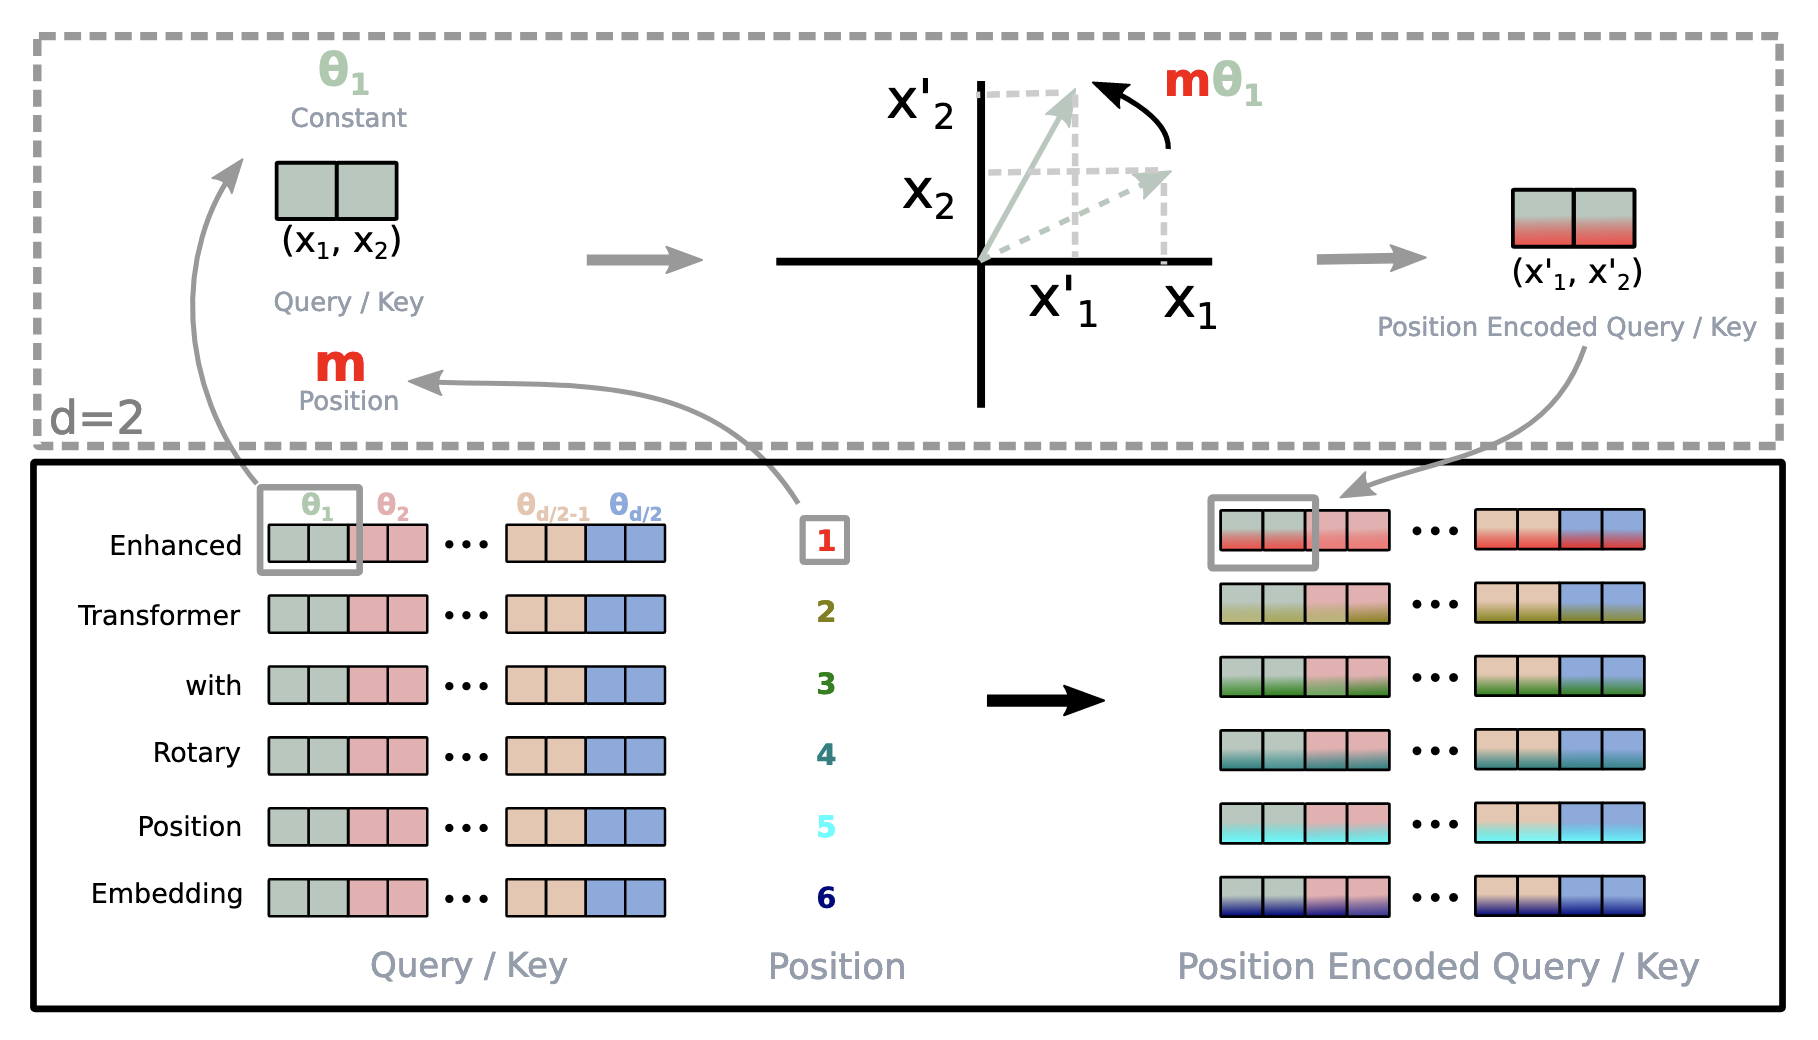
\includegraphics[width=14cm]{figuras/figura-rope.png}
		}{
			}	
	\end{figure}

    \citeonline{dai_rotary_2026} adaptaram o RoPE para processo de pontos, apresentando o \gls{RoTHP}. Isso consistiu em não utilizar mais a posição do indice do token de um modelo de linguagem e sim o timestamp. Um grande benefício dessa abordagem foi tornar a verossimilhança invariante no tempo, pois lida apenas com os tempos relativos (deltas). Isso sugere que se tivermos uma série temporal $\{t_1 + \sigma, t_2+\sigma, \dots, t_n+\sigma\}$ ela vai gerar o mesmo resultado de $\{t_1, t_2, \dots, t_n\}$ e isso resolve um problema de consistência inerente aos modelos que usam tempos absolutos, permitindo time shift.

    As métricas apresentadas nas Tabelas \ref{tab:rothp_nll}, \ref{tab:rothp_accuracy} e \ref{tab:rothp_rmse} demonstram uma clara superioridade do RoTHP em relação à vários modelos tradicionais em vários datasets. Apesar da acurácia estar competitiva com o THP, o avanço foi significativo no calculo da log verossimilhança (NLL) e no RMSE. No RMSE a melhora foi substancial, sobretudo nos datasets do Stack Overflow (SO), onde o RoTHP ultrapassou o THP, que era até então o melhor modelo, em uma margem significativa. Isso sugere que o modelo proposto de rotação de embeddings captura padrões com mais precisão que o encoding senoidal tradicional.
    
    Além disso, parte da robustez do RoTHP advém da sua habilidade de permanecer invariante no tempo. Ao substituir timestamps absolutos para intervalos de tempo através de rotação no plano 2D, o modelo efetivamente conseguiu mitigar o impacto de ruído, muitas vezes causados por problemas de sincronização presentes em datasets reais. Isso mostra que adaptar o RoPE para processos pontuais aumentou a capacidade de generalização dos modelos atuais que utilizam Transformers. Consequentemente, o RoTHP estabelece um novo estado da arte para benchmarks de processos pontuais, até onde nós conhecemos. 

    \begin{table}[h]
        \centering
        \caption{Resultados dos Modelos por Dataset}
        \label{tab:rothp_nll}
        \begin{tabular}{lcccccc}
            \toprule
            \textbf{Models} & \textbf{Financial} & \textbf{SO} & \textbf{Synthetic} & \textbf{Retweet} & \textbf{MemeTrick} & \textbf{Mimic-II} \\ 
            \midrule
            RMTPP   & -3.89  & -2.6   & -1.33 & -5.99 & -6.04 & -1.35 \\
            NHP     & -3.6   & -2.55  & --    & -5.6  & -6.23 & -1.38 \\
            SAHP    & --     & -1.86  & 0.59  & -4.56 & --    & -0.52 \\
            THP     & -1.11  & -0.039 & 0.791 & -2.04 & 0.68  & 0.48  \\
            RoTHP   & 1.076  & 0.389  & 1.01  & 2.01  & 1.71  & 0.64  \\
            \bottomrule
        \end{tabular}
    \end{table} 

    \begin{table}[h]
        \centering
        \caption{Accuracy Comparison}
        \label{tab:rothp_accuracy}
        \begin{tabular}{lccc}
            \toprule
            \textbf{Models} & \textbf{Financial} & \textbf{Mimic-II} & \textbf{SO} \\ 
            \midrule
            RMTPP & 61.95 & 81.2 & 45.9  \\
            NHP   & 62.20 & 83.2 & 46.3  \\
            THP   & 62.23 & 84.9 & 46.4  \\
            RoTHP & 62.26 & 85.5 & 46.33 \\
            \bottomrule
        \end{tabular}
    \end{table}

    \begin{table}[h]
        \centering
        \caption{RMSE Comparison}
        \label{tab:rothp_rmse}
        \begin{tabular}{lccc}
            \toprule
            \textbf{Models} & \textbf{Financial} & \textbf{Mimic-II} & \textbf{SO} \\ 
            \midrule
            RMTPP & 1.56 & 6.12 & 9.78 \\
            NHP   & 1.56 & 6.13 & 9.83 \\
            SAHP  & --   & 3.89 & 5.57 \\
            THP   & 0.93 & 0.82 & 4.99 \\
            RoTHP & 0.60 & 0.57 & 1.33 \\
            \bottomrule
        \end{tabular}
    \end{table}

\section{Length Extrapolation e viés indutivo}\label{sec:length-extrapolation}

Uma limitação comum compartilhada por muitos modelos de sequência baseados em Transformer é sua inabilidade para generalizar sequências mais longas do que aquelas que foram utilizadas durante o treinamento. Esse problema é conhecido como $\textit{length extrapolation}$. Dado um modelo treinado em sequências de tamanho $L_{treino}$, nós verificamos se ele se mantém estável quando testado com sequências de tamanho $L_{teste} > L_{treino}$ \cite{press_train_2021}. A relevância prática dessa limitação é significativa. Em vários cenários do mundo real coletar longas sequências é caro ou mesmo impraticável e, portanto, é desejável treinar em sequências menores e rodar o modelo para ser utilizado em sequências arbitrariamente mais longas. 

A principal causa dessa falha tem sido atribuida à estratégia de  \textit{positional encoding} aplicada nos modelos tradicionais de transformers. Embedding sinusoidal padrão, como introduzido por \citeonline{vaswani_attention_2017} produz representações absolutas dos posicionamentos. Quando o modelo encontra um índice de posição que nunca foi apresentado durante o treinamento, essas representações são efetivamente consideradas \textit{out of distribution}, causando uma rápida degradação de performance, como exposto na seção Resultados. 

\citeonline{press_train_2021} demonstraram empiricamente que modelos sinusoidais são incapazes de extrapolar para sequências maiores que as sequências utilizadas em treinamento, com a métrica de perplexidade aumentando dramaticamente a medida em que $L_{teste}$ cresce. Embeddings rotacionais, como o RoPE \cite{su_roformer_2023}, apresentam melhoras sobre o encoding sinusoidal utilizando encoding relativo, ao invés de posições absolutas. No entanto, \citeonline{press_train_2021} mostraram que mesmo RoPE falha ao extrapolar para sequências substancialmente maiores, como mostra a Figura-\ref{fig:extrapolation-perplexity}.

\begin{figure}
    \centering
    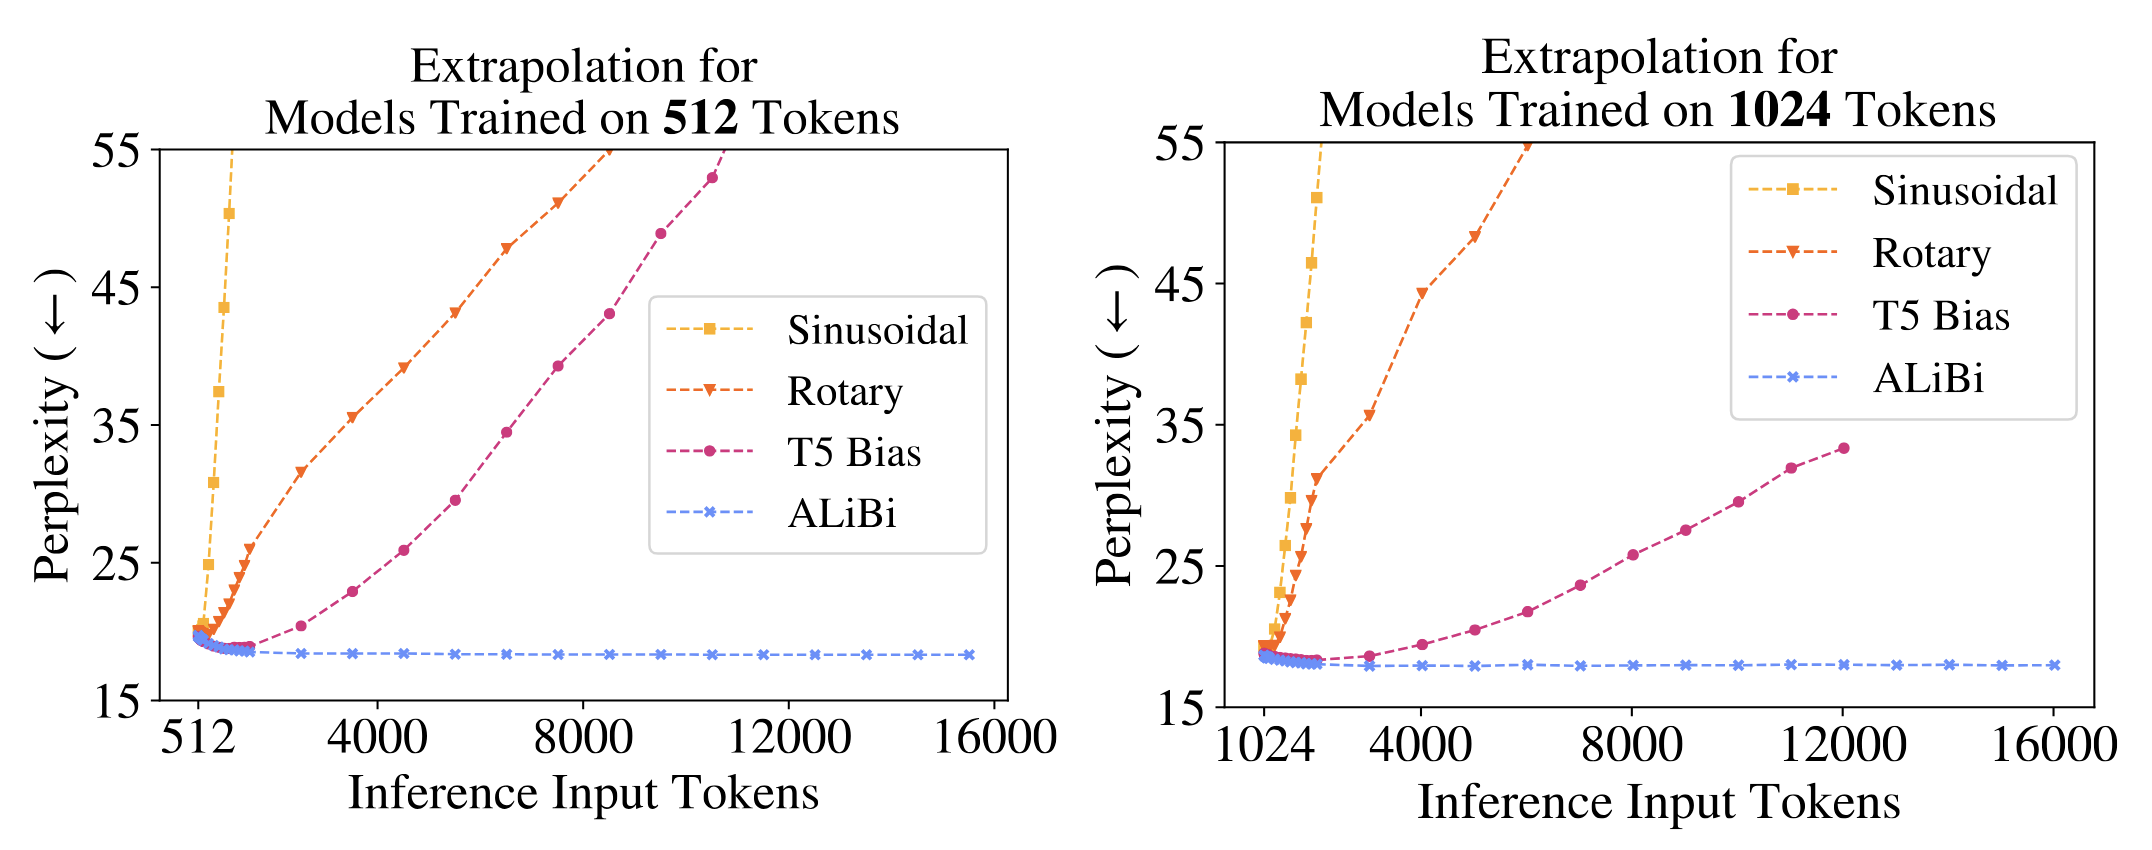
\includegraphics[width=1\linewidth]{figuras/fig_extrapolation_perplexity.png}
    \caption{A medida em que a extrapolação aumenta, percebemos claramente que a degradação demonstrada pelo RoPE é menor que a de métodos tradicionais sinusoidais, mas ainda assim muito mais acentuada que o modelo proposto por \citeonline{press_train_2021}}
    \label{fig:extrapolation-perplexity}
\end{figure}

\subsection{Attention with Linear Biases (ALiBi)}\label{subsec:alibi}

\citeonline{press_train_2021} propuseram uma abordagem fundamentalmente diferente do positional encoding. Ao invés de adicionar ou rotacionar embeddings, eles introduziram uma penalidade estática, não aprendível, diretamente no escore de atenção. Esse método, chamado \textit{Attention with Linear Biases (ALiBi)}, substitui o passo do positional embedding completamente. A motivação principal do modelo é que ele deve dar menos importância para tokens a medida em que eles vão se distanciando do índice atual, os autores chamam de \textit{inductive bias towards recency}. Ao invés de aprender essa propriedade a partir dos dados, o ALiBi computa esse decaimento de "importância" em sua própria arquitetura. 

Em modelos tradicionais de transformers, position embeddings são adicionados nos embeddings das palavras (tokens). O produto escalar dos vetores Q e K é computado da seguinte forma:
\begin{equation}
    \text{softmax}\!\left(q_i K^\top\right),
\end{equation}
onde o resultado é então multiplicado pelos valores de $V$. O ALiBi apenas modifica o passo após o produto escalar, deixando todo o resto intacto: 
\begin{equation}
    \text{softmax}\!\left(q_i K^\top + m \cdot \left[-(i-1), \ldots, -2,-1,\; 0\right]\right),
    \label{eq:alibi}
\end{equation}
onde o vetor $[-(i-1), \ldots, -2, -1, 0]$ representa as distâncias de cada posição K para a posição Q corrente $i$ e o escalar $m$ é um coeficiente de inclinação específico por cabeça de atenção, fixado antes do treinamento e nunca é atualizado. O sinal negativo garante que a penalidade diminui o attention score a medida em que a distância entre Q e K aumentam, efetivamente suprimindo a atenção para tokens distantes. Para um modelo com $n$ cabeças de atenção, a inclinação $m$ forma uma progressão geométrica com razão e primeiro termo ${2^{\frac{-8}{n}}}$ \cite{press_train_2021}.

\subsection{Viés indutivo e sua relevância no Processo de Hawkes}
\label{subsec:inductive-bias-hawkes}

Um viés indutivo é uma afirmação que guia o modelo, independente dos dados treinados. No contexto posicional do ALiBi, podemos afirmar que o viés indutivo dita que palavras/tokens distantes são menos relevantes, linearmente, que quando mais próximas. A penalidade é aplicada diretamente no código, e não apenas nos dados aprendidos. 

O viés indutivo não é arbitrário. Na verdade, ela está presente no Processo de Hawkes desde sua proposição, em 1971. Olhando para a equação do Processo Hawkes, a influência de um evento passado $t_i$ decai a medida em que o intervalo $t - t_i$ aumenta, na proporção de $\beta$. Quanto maior a distância, menor a contribuição do evento para o processo. Isso mostra que o Processo de Hawkes possui em sua essência um viés indutivo representado pelo parâmetro exponencial de decaimento. 

O THP e o RoTHP substituem o kernel paramétrico de Hawkes por um mecanismo de atenção. Isso trouxe enormes vantagens para esses modelos, como a possibilidade de capturar relações mais complexas, e inclusive invariância temporal, no caso do RoTHP, mas o preço pago foi se distanciar da equação formal do processo de Hawkes original. 

O mecanismo de atenção não impõe nenhuma amarra sobre como ela deve considerar a distância entre os tokens, no caso de um TPP, dos eventos. Qualquer decaimento que emerge do modelo é resultado do aprendizado realizado com os dados e não uma garantia estrutural. Inclusive, pela natureza oscilatória do calculo sinusoidal, por ocasião eventos distantes podem receber mais relevância que eventos próximos.